\documentclass[conference,letterpaper]{IEEEtran}
\usepackage[T1]{fontenc}
\usepackage[utf8]{inputenc}
\usepackage{cite}
\usepackage{amsmath,amssymb}
\usepackage{booktabs}
\usepackage{pgfplots}
\pgfplotsset{compat=1.18}
\usepackage{tikz}
\usetikzlibrary{positioning,arrows.meta}
\usepackage{xurl}
\usepackage[hidelinks]{hyperref}
\title{Sentiment, Troubleshooting, and Evidence\\
in Reddit Software-Update Discussions}
\author{\IEEEauthorblockN{Manu Mathew Jiss and Solomon Berhe}
\IEEEauthorblockA{School of Engineering and Computer Science\\
University of the Pacific, Stockton, California, USA\\
m\_jiss@u.pacific.edu, sberhe@pacific.edu}}
\begin{document}
\maketitle
\begin{abstract}
Negative tone, troubleshooting purpose, visible diagnostic facts, and a reviewer's first action are distinct descriptions of a Reddit software-update post. On a later fresh test, title-and-body text reaches macro-F1 0.792. Adding general or software-engineering sentiment scores to development text brings no reliable gain over text alone. Reproduction context and error evidence are often missing. Two reviewers chose different first actions in 9 of 30 cases. The study does not evaluate a triage pipeline.
\end{abstract}
\begin{IEEEkeywords}
software updates, Reddit, sentiment analysis, troubleshooting, diagnostic evidence
\end{IEEEkeywords}

\section{Introduction}
Users report crashes, changed behavior, and design disagreement after updates \cite{Hassan2020BadUpdates}. Teams still struggle to interpret that feedback during continuous delivery \cite{Tkalich2025Feedback}. Forums and Reddit threads are one place the reports appear \cite{Iqbal2021Reddit}, \cite{Tizard2019Forums}, \cite{Singh2024ReleaseNotes}. A negative tone does not establish a fault report \cite{Jongeling2017Negative}, \cite{Lin2018HowFar}. A troubleshooting label does not establish that the saved text contains the facts a bug report is expected to carry \cite{Bettenburg2008GoodReport}, \cite{Chaparro2017Missing}. And a purpose label does not choose the next engineering action.

Our central question is how an informal software-update discussion can become useful engineering evidence. We answer it by keeping four descriptions separate. \textbf{RQ1:} Within posts already judged to concern software and an update, how well does title-and-body text distinguish troubleshooting from other update discussion on held-out posts? \textbf{RQ2:} On the Reddit-URL development set, how much of that distinction is in the title, the body, or a sentiment score, and does a valence gap remain under a dissatisfaction-only negative class or under a secondary cohort with different assigned labels? \textbf{RQ3:} Which diagnostic facts are visible in a reviewed sample of troubleshooting posts? \textbf{RQ4:} How do two reviewers explain first-pass actions on 30 intact posts? Together these questions test where a post's tone, purpose, facts, and possible response agree or separate. They do not form a tested causal workflow. The contribution is an empirical boundary: sentiment is a weak proxy for troubleshooting in this task, and identifying troubleshooting does not certify that its evidence supports a particular action.

\section{Related Work}
Hutto and Gilbert published VADER for short social-media text \cite{Hutto2014VADER}. Islam and Zibran built SentiStrength-SE because general lexicons misread software wording \cite{Islam2018SentiStrengthSE}. Calefato et al.\ trained Senti4SD on developer communication \cite{Calefato2018Senti4SD}. Lin et al.\ reported negative results after retraining \cite{Lin2018HowFar}. Jongeling et al.\ showed that the choice of sentiment tool can change a study's conclusion \cite{Jongeling2017Negative}. Novielli et al.\ extended that warning to software-engineering tools used off the shelf \cite{Novielli2021Replication}. Cassee et al.\ show that transformer models and tokenization choices change sentiment estimates on software-engineering text \cite{Cassee2024Transformers}. We score four frozen sentiment numbers on the same development text: VADER, TextBlob, a social-media RoBERTa sentiment checkpoint, and the official SentiStrength-SE v1.5 dictionary \cite{SentiStrengthSETool}. None is fine-tuned here or a troubleshooting label. An official Senti4SD comparison was attempted, but its required pretrained artifacts could not be retrieved, so no score is reported. A null increment for these four tools is not a claim about every software-engineering sentiment model.

Forum studies treat conversational posts as a source of requirements and development insight, while warning that the insight is mixed with other talk \cite{Tizard2019Forums}, \cite{Wang2024Forums}, \cite{Iqbal2021Reddit}. Issue-report studies document which elements developers say they need, including reproduction steps and traces, and how often those elements are missing \cite{Bettenburg2008GoodReport}, \cite{Chaparro2017Missing}, \cite{Soltani2020Elements}, \cite{Wang2025InformationNeeds}. Feedback classifiers can also move when the dataset changes \cite{Devine2023Transfer}. Mapping and industrial studies treat practitioner judgment as a separate question from classifier accuracy \cite{Laiq2026Mapping}. ChatBR detects missing report components and proposes additions \cite{Bo2024ChatBR}. Wang et al.\ evaluate an agent-governed workflow that turns noisy feedback into evidence-aware issue specifications \cite{Wang2026Evidence}. That paper tests an end-to-end specification process. This one does not. We do not retrieve, generate, or score a repaired report. We record whether selected facts are visible in the saved snapshot, and we record how two reviewers explain a first action. The two descriptions stay separate from the purpose score.

\section{Sources and Populations}
Candidate posts were retrieved through \mbox{ReleaseTrain} \cite{ReleaseTrainDocs}. The saved \texttt{/api/reddit/query/tps} and \texttt{/query/gds} responses are candidate pools, not confirmed labels. Raw responses for the secondary cohort were saved on 27~March~2026. Later candidate pages were saved on 5~October~2026. A post uses the October snapshot when one exists and the March snapshot otherwise. Snapshots are not concatenated, and no live page was fetched for this analysis.

The combined collection has 3,362 records. It is not a verified-Reddit census: the development slice contains 30 records whose URL metadata are not Reddit. Primary purpose and sentiment results use the 2,050 Reddit-URL development rows. The scored tests were checked separately against saved URL fields, not inferred from community names. All 159 reserved rows have a \texttt{reddit.com} URL in the combined collection, and the same host in the later saved collection pages. All 344 fresh rows are outside the combined collection; each has a \texttt{reddit.com} URL in the saved fresh-collection pages. Neither scored test includes the 30 non-Reddit URL records. Table~\ref{tab:pop} lists every denominator below.

The current negative class is other update discussion: 392 of the 2,050 posts, of which 68 are assigned general dissatisfaction and 324 have another discussion type. The secondary cohort's negative class is assigned general dissatisfaction (456 of 542). Those label systems answer different questions and are not pooled. Class proportions in either set are not prevalence estimates. Figure~\ref{fig:design} shows the analyses as branches. A line means that an analysis uses those records. It does not mean that sentiment, a purpose score, or a diagnostic code determines a reviewer action.

\begin{figure*}[t]
\centering
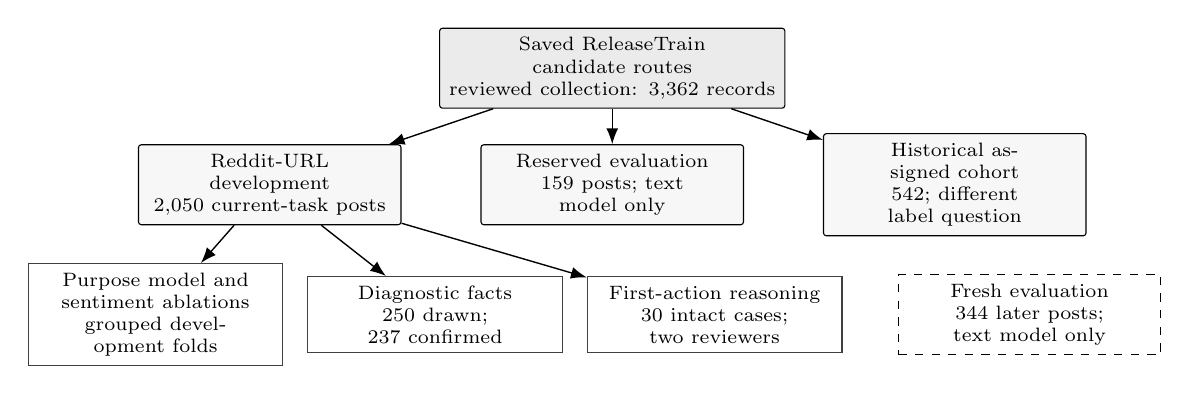
\begin{tikzpicture}[
  font=\scriptsize,
  source/.style={draw=black, fill=black!8, rounded corners=1pt,
    align=center, minimum height=0.8cm, text width=4.15cm},
  set/.style={draw=black, fill=black!3, rounded corners=1pt,
    align=center, minimum height=0.91cm, text width=3.10cm},
  analysis/.style={draw=black!75, align=center, minimum height=0.82cm,
    text width=3.0cm},
  external/.style={draw=black, dashed, align=center,
    minimum height=0.91cm, text width=3.10cm},
  flow/.style={-{Latex[length=2mm]}, line width=0.5pt}
]
\node[source] (col) at (0,0) {Saved ReleaseTrain candidate routes\\reviewed collection: 3,362 records};
\node[set] (dev) at (-4.35,-1.48) {Reddit-URL development\\2,050 current-task posts};
\node[set] (res) at (0,-1.48) {Reserved evaluation\\159 posts; text model only};
\node[set] (sec) at (4.35,-1.48) {Historical assigned cohort\\542; different label question};
\node[analysis] (cls) at (-5.8,-3.13) {Purpose model and sentiment ablations\\grouped development folds};
\node[analysis] (diag) at (-2.25,-3.13) {Diagnostic facts\\250 drawn; 237 confirmed};
\node[analysis] (case) at (1.3,-3.13) {First-action reasoning\\30 intact cases; two reviewers};
\node[external] (fresh) at (5.30,-3.13) {Fresh evaluation\\344 later posts; text model only};
\draw[flow] (col) -- (dev);
\draw[flow] (col) -- (res);
\draw[flow] (col) -- (sec);
\draw[flow] (dev) -- (cls);
\draw[flow] (dev) -- (diag);
\draw[flow] (dev) -- (case);
\end{tikzpicture}
\caption{Data provenance and separate analyses. Branches may overlap and are not an additive partition. Solid arrows mean that records were used in an analysis, not that one analysis caused the next. The fresh test was collected outside the 3,362 records; its dashed box has no parent arrow. Diagnostic coding and first-action review are sibling analyses rather than outputs of the classifier.}
\label{fig:design}
\end{figure*}

\begin{table}[t]
\caption{Populations used below. Test scores are text-only.}
\label{tab:pop}
\centering
\footnotesize
\setlength{\tabcolsep}{3pt}
\begin{tabular}{lrrl}
\toprule
Population & Rows & Pos. & Negative class \\
\midrule
Combined collection & 3,362 & --- & Mixed sources \\
Reddit-URL development & 2,050 & 1,658 & 392 other update \\
\quad dissatisfaction type & 68 & 0 & Inside the 392 \\
\quad other type & 324 & 0 & Inside the 392 \\
Non-Reddit URL records & 30 & 28 & Excluded \\
Secondary assigned cohort & 542 & 86 & 456 dissatisfaction \\
Reserved test & 159 & 135 & 24 other update \\
Fresh test & 344 & 277 & 67 other update \\
Diagnostic draw & 250 & --- & Then reconfirmed \\
Diagnostic confirmed & 237 & 237 & Troubleshooting only \\
Intact cases & 30 & --- & Exploratory \\
\bottomrule
\end{tabular}
\end{table}

\section{Methods}
\subsection{Annotation and provenance}
A current-task label requires a reviewed software scope and an update connection. The positive class is troubleshooting. Review provenance for the full collection is mixed: some portions were reviewed with assistance, some were reviewed jointly, and some were held for pilots or protected tests. We therefore do not call the collection an independent gold set, and we do not revise stored labels after test scores were known. The fresh-test labels are a user-reported joint review; the saved freeze record states that no independent first-pass agreement can be estimated from the files. The diagnostic sample is also a joint review record and has no separate field-level agreement statistic. The 30-case record states that two reviewers with software-engineering knowledge completed separate first passes. No field records that a comment resolved a problem. Absence of such a field is an unknown outcome.

The \texttt{releasetrain-sentiment} 0.2.1 package was inspected and not used. Its author average is the mean of stored author comments, or zero when none is stored. The secondary-cohort trajectories can use the post title in that case. Those two constructions are not interchangeable.

\subsection{Purpose classifier and grouped thresholds}
The text model is word and bigram TF--IDF, minimum document frequency 2, at most 20,000 features, and sublinear term frequency, followed by class-balanced logistic regression with $C=4$, the liblinear solver, and random state 42. The vectorizer is fit inside each training fold. Near-duplicate posts stay together: groups are the union of pairs whose normalized title-plus-body character five-gram Jaccard is at least 0.92. Development scores use five-fold stratified group splits with shuffle and seed 42.

For the development comparisons in RQ2, the decision threshold is chosen only on the outer training split. Three inner stratified group folds, also seed 42, score a grid from 0.20 to 0.80 in steps of 0.05. The selected cutoff maximizes mean inner macro-F1, then mean inner F1 of the other-update class, then closeness to 0.5. Outer-fold labels never choose the cutoff. The reserved and fresh tests use one previously fixed specification and the saved continuity threshold 0.588. They were not rescored for this paper, and sentiment features were not attached to them. Fresh majority and fixed-keyword scores come from the same saved test file. The fixed-keyword rule looks for predefined malfunction and recovery cues. It is a text heuristic, not a sentiment model.

\subsection{Sentiment construction}
VADER 3.3.2 supplies the compound score \cite{Hutto2014VADER}. On title and body, the input is the raw title, a newline, and the raw body. An empty or whitespace document returns 0.0, which collides with genuine neutral text. On the 2,050 Reddit-URL posts, 303 bodies are empty and 237 title-body compounds are exactly zero. The primary comparison adds only that one compound to the same title-and-body string. The first comparison is therefore text versus the same text plus one sentiment column. The same protocol, and the same grouped folds, then score three further sentiment numbers and one frozen embedding. TextBlob 0.20.1 supplies polarity on the same raw title, newline, and body. The contextual score is $P(\mathrm{positive})-P(\mathrm{negative})$ from the frozen checkpoint \texttt{cardiffnlp/\allowbreak twitter-roberta-\allowbreak base-sentiment-latest}, truncated at 512 tokens. Neutral probability stays in the distribution and is not added. SentiStrength-SE v1.5 supplies a positive and a negative strength from its packaged software-engineering dictionary \cite{SentiStrengthSETool}; we add the signed strengths to form one polarity feature. Because its command-line interface scores one document per line, embedded title-body line breaks and tabs become spaces. There is no sentiment gold label on these posts, so a sentiment-only arm is not a check that the number matches a human valence judgment. A frozen MiniLM encoder (\texttt{all-MiniLM-L6-v2}) supplies normalized embeddings to a class-balanced logistic regression with $C=1$. The encoder is not fine-tuned. Each augmented arm adds one score to the same title-and-body TF--IDF features. Scalers, like vectorizers, are fit on the training fold only. Title-only and body-only ablations use the same classifier and inner thresholds; a missing body stays an empty string, and those posts are not dropped. None of these development arms was scored on the reserved or fresh tests.

A second comparison is limited to the 797 Reddit-URL posts with at least one nonempty stored comment. Both models see one full-thread string: the chosen snapshot title, the body, then nonempty comments in timestamp order. The augmented model adds the title-body compound, the mean of author comments or zero, the mean of community comments or zero, and two missingness flags. An author comment is marked by the stored submitter flag or an author-name match. The title is not used as an author-comment fallback in this comparison. All 7,388 nonempty comments in that subset have timestamps at or after the post, so the features are retrospective. A predeclared bar for a strong comment-feature claim required both an author comment and a community comment on at least half of the 2,050 posts. The observed both-role count is 466 (22.7\%), so comment models stay limited descriptions.

Paired differences are macro-F1 of the augmented model minus macro-F1 of the text model. Intervals use 1,000 bootstrap resamples with seed 42, both by post and by duplicate group. A keyword-first rule that returns troubleshooting whenever technical cues are present is reported only as a heuristic.

Comment storage is uneven (Table~\ref{tab:cov}). On the 2,050 Reddit-URL posts, 797 have a nonempty stored comment: 560 troubleshooting and 237 other-update. Author replies are stored for 362 troubleshooting and 112 other-update posts; community comments for 554 and 235; both roles for 356 and 110. No stored comment remains for 1,098 of 1,658 troubleshooting posts and 155 of 392 other-update posts. The 30 non-Reddit URL records contribute no comments. Coverage is a property of the snapshot, not of the live thread.

\begin{table}[t]
\caption{Stored-comment coverage on 2,050 Reddit-URL posts.}
\label{tab:cov}
\centering
\footnotesize
\setlength{\tabcolsep}{4pt}
\begin{tabular}{lrr}
\toprule
Stored text & Trouble & Other \\
\midrule
Nonempty comment & 560 & 237 \\
Author reply & 362 & 112 \\
Community comment & 554 & 235 \\
Both roles & 356 & 110 \\
No stored comment & 1,098 & 155 \\
\bottomrule
\end{tabular}
\end{table}

\subsection{Fine-tuned purpose comparator}
We fine-tune \texttt{roberta-base} \cite{Liu2019RoBERTa} on the same 2,050 development posts and five duplicate-group folds. A grouped inner split chooses one to three epochs and a threshold; a fresh model refit on each full outer-training fold is scored once. Settings are seed 42, 256 tokens, batch 8, AdamW at $2\times10^{-5}$, and no class weights. Later text is truncated in 442 posts (22\%). Neither protected test is used.

\subsection{Diagnostic codebook}
The diagnostic sample is a simple random draw of 250 posts from the then-current 1,658 Reddit-URL troubleshooting development rows, taken before the diagnostic answers. A 50-post feasibility exercise and a 15-post rule check preceded the frozen guide and are not added into the 250. Ten sampled posts overlapped that earlier exercise by chance; their main-study answers were recorded separately under the final guide.

Coders read only the saved title and body. Community name, candidate route, old labels, model scores, comments, and live pages were out of scope. The first decision reconfirmed troubleshooting: yes, no, or unclear. Field summaries are conditional on yes. Eight fields were then marked present, not observed, or unclear: software product, identifiable release, environment, specific symptom, reproduction context, error evidence, attempted remedy, and an explicit help request. An identifiable release needs a version, build, named release, or unambiguous cycle; ``latest update'' alone is not enough. Reproduction context needs an action or condition, not timing alone. Error evidence needs a specific message, code, log, trace, or described diagnostic output. An image that is referenced but unreadable can make that field unclear. A remedy must have been attempted. Not observed means not visible in the snapshot. It is not proof that the fact was absent from the incident. No overall usefulness score was assigned. The 13 posts marked no or unclear stay in the classifier snapshot; diagnostic exclusion does not relabel them. Table~\ref{tab:code} records the present-rule used for each field. The same guide states that a blank body does not automatically make every field unclear.

\begin{table}[t]
\caption{Present-rule for the eight diagnostic fields. Not observed means not visible in the saved title or body.}
\label{tab:code}
\centering
\footnotesize
\setlength{\tabcolsep}{3pt}
\begin{tabular}{lp{4.6cm}}
\toprule
Field & Counted present when the text gives \\
\midrule
Product & An app, OS, service, tool, or component \\
Release & A version, build, named release, or unique cycle \\
Environment & A device, OS, host, or configuration \\
Symptom & Concrete wrong behavior \\
Reproduction & An action or condition for that behavior \\
Error evidence & A message, code, log, trace, or described output \\
Remedy & A fix or workaround actually tried \\
Help request & An explicit request for diagnosis or a fix \\
\bottomrule
\end{tabular}
\end{table}

\subsection{Thirty intact cases}
After a six-post pilot, excluded from the counts, two reviewers read 30 purposefully selected intact title-and-body snapshots. The cases were varied by community, update situation, symptom, evidence, and expected difficulty. Each reviewer chose one first action: open an update-focused investigation, request a specific clarification, monitor or group similar reports, take no update-focused action, or mark the case unassessable. They also named the evidence they used. The assigned discussion label was hidden. Counts describe these 30 cases and these two readers only. They were not crossed with VADER scores, and they are not a population rate. Saved identifiers show that the 30 are not a subset of the 237: six main-case rows also appear in the confirmed diagnostic sample, and the case list was not drawn from that sample. The six pilot cases are excluded from the counts.

\section{Results}
\subsection{Purpose detection}
Table~\ref{tab:purpose} reports the saved text-only tests. Fresh macro-F1 is 0.792, above the fresh majority score of 0.446 and the fixed-keyword score of 0.474. The fresh confusion matrix is 46 of 67 other-update posts and 252 of 277 troubleshooting posts correct. Other-update F1 on that test is 0.667. The reserved score is 0.863, with 18 of 24 other-update posts and 130 of 135 troubleshooting posts correct, and other-update F1 0.766. The two tests use the same specification and different fitted training populations, so the drop is descriptive rather than a controlled transfer estimate. Framing these evaluations with the later sentiment and case analyses does not raise either score.

On the 2,050-post development text, the same grouped protocol gives logistic regression macro-F1 0.831932. A linear SVM with the same TF--IDF and its default margin scores 0.820. A keyword-first heuristic scores 0.685. Multinomial naive Bayes, which is not class-balanced in this run, scores 0.551 and predicts every troubleshooting post as troubleshooting (confusion 43 and 349 on the other-update class, and 0 and 1,658 on troubleshooting). These are text baselines. They are not evidence that a sentiment feature helps.

On those folds, RoBERTa scores macro-F1 0.839 versus 0.832 for TF--IDF (difference $+0.007$; paired duplicate-group 95\% interval $-0.016$ to $+0.029$). The interval includes zero. Other-update F1 is 0.737 versus 0.729, but recall is lower (0.709 versus 0.737). RoBERTa fixes 119 text-model errors and introduces 102; inner thresholds span 0.35--0.80. Neither protected test was rescored.

Title and body are not substitutes for each other (Table~\ref{tab:ablate}). Title only scores 0.750534 and body only 0.781424. Against title and body together, the grouped 95\% intervals for those drops are $-0.107$ to $-0.057$ and $-0.069$ to $-0.032$. Both exclude zero. Of the 2,050 posts, 303 have an empty body: 177 other-update and 126 troubleshooting. Those rows stay in every arm as empty strings. The class mix differs, so an empty body is not by itself an explanation of an error.

Adding a VADER compound computed from only the same input changes title-only macro-F1 by $+0.0003$ and body-only by $+0.0046$. The paired duplicate-group intervals are $[-0.014,0.016]$ and $[-0.005,0.014]$; both include zero. Using sentiment from the full title and body to augment a title-only or body-only arm would have leaked excluded text into that arm, so we do not do so.

To inspect what the linear model uses, we refit it on each outer training fold and recorded the 25 largest coefficients in each direction without consulting that fold's held-out labels. Some terms recur in all five lists (Fig.~\ref{fig:terms}). Words such as \emph{error}, \emph{fix}, and \emph{tried} are consistent with a help-seeking report; \emph{released} and \emph{features} are consistent with update news. Function words and platform names also rank highly. These are associations with assigned labels, not independent evidence that the model understood an incident or that a term caused its prediction.

\begin{figure}[t]
\centering
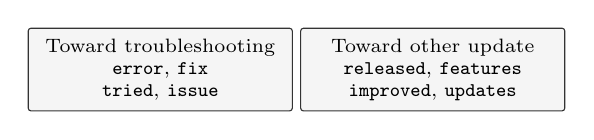
\begin{tikzpicture}[font=\scriptsize,
  cue/.style={draw=black!80, fill=black!4, rounded corners=1pt,
    align=center, text width=3.12cm, minimum height=1.05cm}]
\node[cue] at (-1.73,0) {Toward troubleshooting\\\texttt{error}, \texttt{fix}\\\texttt{tried}, \texttt{issue}};
\node[cue] at (1.73,0) {Toward other update\\\texttt{released}, \texttt{features}\\\texttt{improved}, \texttt{updates}};
\end{tikzpicture}
\caption{Illustrative lexical cues from the TF--IDF model. Every displayed term appeared among the 25 largest coefficients in its direction in all five outer-training fits. The display is selective, not a ranked importance estimate or a causal explanation; other high-weight terms include function words and platform names.}
\label{fig:terms}
\end{figure}

\begin{table}[t]
\caption{Text-only purpose scores. Development rows use grouped out-of-fold predictions; test rows are the earlier protected evaluations. No sentiment feature is included.}
\label{tab:purpose}
\centering
\footnotesize
\begin{tabular}{lrl}
\toprule
Evaluation & $n$ & Macro-F1 \\
\midrule
Development TF--IDF & 2,050 & 0.832 \\
Development RoBERTa & 2,050 & 0.839 \\
Reserved test & 159 & 0.863 \\
Fresh test & 344 & 0.792 \\
Fresh majority & 344 & 0.446 \\
Fresh fixed keyword & 344 & 0.474 \\
\bottomrule
\end{tabular}
\end{table}

\subsection{Where valence separates, and where it does not}
On all 2,050 Reddit-URL posts, text macro-F1 is 0.831932 and the same text plus the title-body compound is 0.833130 (Table~\ref{tab:sent}). The difference is $+0.001$. The post-level 95\% interval is $-0.012$ to $+0.015$, and the duplicate-group interval is $-0.013$ to $+0.015$. Both include zero. Other-update F1 changes by $+0.001$, and that interval also includes zero. VADER alone scores 0.533519, above the majority baseline of 0.447 but well below text. TextBlob alone scores 0.552128, and the same text plus polarity scores 0.834445 (group interval $-0.008$ to $+0.015$). The frozen contextual score alone is 0.783792. Added to the same text it scores 0.835524 (group interval $-0.022$ to $+0.027$). SentiStrength-SE alone scores 0.464797, with other-update F1 only 0.057; with the same text it scores 0.834083 (group interval for the increment $-0.004$ to $+0.009$). All four augmented group intervals include zero. The contextual model truncated 188 of the 2,050 texts at 512 tokens; the median length is 134 tokens. Truncation can drop later body text from that score only. It does not change the TF--IDF arms. No sentiment gold label exists for these posts, and none of the new arms was applied to the reserved or fresh tests.

A frozen MiniLM head on the same folds scores 0.847561, which is $+0.016$ relative to title and body. The grouped interval is $-0.009$ to $+0.039$ and includes zero, as does the post-level interval. The point estimate is higher. It is not evidence that the embedding is superior on this task. The classifier is using lexical purpose cues. A sentiment number does not add a reliable increment.

The inner-threshold title-and-body predictions on these 2,050 posts are 289 true negatives, 103 false positives, 112 false negatives, and 1,546 true positives. Among the 303 empty-body posts, 17 of 177 other-update posts are false positives and 40 of 126 troubleshooting posts are false negatives. Among posts with a body, the corresponding counts are 86 of 215 and 72 of 1,532. Empty-body posts are mostly other-update, so those rates are not a cause. Four errors are paraphrased only as illustrations. They were not re-adjudicated, and the selection is not a frequency. A title-only cluster-upgrade failure, assigned troubleshooting, was predicted as other update. A title-only note that a keyboard emoji panel looks cleaner after an update, assigned other update, was predicted as troubleshooting. A long complaint that one phone overheats and freezes after interface updates, stored as general dissatisfaction and therefore other update, was predicted as troubleshooting. A report that system updates crash a pen-enabled laptop, together with a request for advice on changing operating systems, was assigned troubleshooting and predicted as other update.

Figure~\ref{fig:valence} shows why a class-mean plot can still look informative. Mean title-body VADER compound is $-0.064$ for troubleshooting ($n=1{,}658$) and $+0.194$ for the pooled other-update class ($n=392$). Splitting that negative class, the 324 posts of type \texttt{other} have mean $+0.249$, while the 68 dissatisfaction posts have mean $-0.068$. The VADER troubleshooting-minus-dissatisfaction difference is $+0.004$, and its interval includes zero. Text classification of that 1,726-post pair reaches macro-F1 0.658 because the classes are highly unbalanced; adding the compound changes it by $+0.010$, and that interval includes zero. VADER alone predicts every one of those 1,726 posts as troubleshooting. For VADER, the apparent pooled gap is thus not a gap against confirmed dissatisfaction. Much of the positive mass sits in update talk that was not labeled as dissatisfaction.

An exploratory slice after the SentiStrength-SE comparison gives a different descriptive result. Its signed-strength mean is $-0.027$ for troubleshooting, $-0.794$ for the 68 dissatisfaction posts, and $+0.139$ for other discussion. The troubleshooting-minus-dissatisfaction difference is $+0.767$ (duplicate-group bootstrap interval $+0.481$ to $+1.055$): this tool calls dissatisfaction markedly more negative than troubleshooting. The two scores use different scales and should not be compared by magnitude. The disagreement in direction of the within-class contrast is a reason to avoid treating one automatic sentiment score as a universal definition of the task. SentiStrength-SE still adds no reliable predictive gain to title-and-body text (Table~\ref{tab:sent}).

A closed-list description on the same 2,050 posts points the same way and is not a causal mask. Incident terms appear in 1,258 of 1,658 troubleshooting posts (76\%) and in 154 of 392 other-update posts (39\%). Discontent terms appear in about 10\% and 11\% of those classes. Posts with discontent terms and no incident terms are few: 33 troubleshooting posts, mean compound $-0.275$, and 13 other-update posts, mean $-0.223$. Technical wording and evaluative wording are not the same partition as the purpose label.

\begin{table}[t]
\caption{Development macro-F1 on 2,050 grouped folds. Sentiment-only arms see one score. Augmented arms add that score to title and body.}
\label{tab:sent}
\centering
\footnotesize
\setlength{\tabcolsep}{3pt}
\begin{tabular}{lrr}
\toprule
Arm & Alone & With text \\
\midrule
Title and body & 0.831932 & --- \\
VADER compound & 0.533519 & 0.833130 \\
TextBlob polarity & 0.552128 & 0.834445 \\
Contextual score & 0.783792 & 0.835524 \\
SentiStrength-SE & 0.464797 & 0.834083 \\
Frozen MiniLM head & --- & 0.847561 \\
\bottomrule
\end{tabular}
\end{table}

\begin{table}[t]
\caption{Input ablation on the same 2,050 posts and folds. Each VADER score uses only that arm's input; empty bodies are retained.}
\label{tab:ablate}
\centering
\footnotesize
\begin{tabular}{lr}
\toprule
Input & Macro-F1 \\
\midrule
Title and body & 0.831932 \\
Title only & 0.750534 \\
Title + title VADER & 0.750843 \\
Body only & 0.781424 \\
Body + body VADER & 0.786073 \\
\bottomrule
\end{tabular}
\end{table}

\begin{figure}[t]
\centering
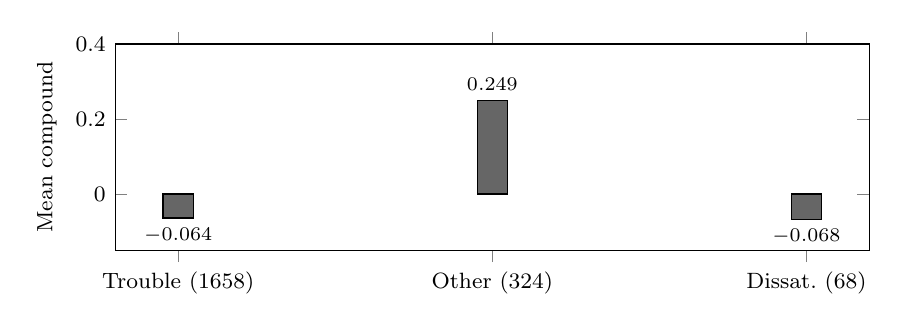
\begin{tikzpicture}
\begin{axis}[
    ybar,
    width=0.92\columnwidth,
    height=4.2cm,
    ymin=-0.15, ymax=0.40,
    ylabel={Mean compound},
    ylabel style={font=\footnotesize},
    symbolic x coords={T,O,D},
    xtick=data,
    xticklabels={Trouble (1658),Other (324),Dissat.\ (68)},
    x tick label style={font=\footnotesize},
    y tick label style={font=\footnotesize},
    bar width=11pt,
    nodes near coords,
    every node near coord/.append style={font=\scriptsize, /pgf/number format/fixed, /pgf/number format/precision=3},
]
\addplot[fill=black!60] coordinates {(T,-0.064) (O,0.249) (D,-0.068)};
\end{axis}
\end{tikzpicture}
\caption{Mean title-body VADER compound on the 2,050 Reddit-URL development posts, split by assigned discussion type. Trouble and Dissat.\ are close. The positive mean is the other discussion type inside the current negative class. The panel is descriptive, not a causal contrast.}
\label{fig:valence}
\end{figure}

Among 797 posts with a stored comment, full-thread text scores 0.866 and the same text plus sentiment columns scores 0.839. The difference is $-0.027$. Post-level and group-level intervals both exclude zero on this subset (group interval $-0.051$ to $-0.005$). Only 14 of the 797 posts share a duplicate group, so that exclusion is a weak dependence correction, not a general claim that sentiment features harm classification. Stored comments are missing for 1,098 of 1,658 troubleshooting posts (66\%) and for 155 of 392 other-update posts (40\%). All 30 non-Reddit URL records lack a stored comment. The lower thread score is a selected, retrospective result.

The secondary cohort has 86 posts assigned as technical problem statements and 456 assigned as general dissatisfaction. Full-file author--community divergence is 0.371 versus 0.287 (Mann--Whitney $p=0.009$). Author means are 0.009 versus 0.191; community means are 0.168 versus 0.194 (Welch $p=0.33$). Author tracks use the title alone for 205 posts. After those tracks are removed, author means remain lower for the technical class (0.077 versus 0.261), but divergence is no longer distinguished at $p=0.05$ ($p=0.060$). Author slope is not significant. This cohort uses a different label system from the 2,050-post task, including the 68-post dissatisfaction slice of that task.

\subsection{Diagnostic visibility}
Reconfirmation of the 250-post draw kept 237 troubleshooting posts, marked four as not troubleshooting, and left nine unclear. Table~\ref{tab:fields} and Figure~\ref{fig:fields} use the signed conditional counts on those 237. A specific symptom is recorded for every retained post, which partly follows from reconfirming the troubleshooting designation. Error evidence is present in 40 posts (16.9\%; Wilson 12.6--22.2\%). Seven further error-evidence decisions were unclear and are not counted as absence. Reproduction context is present in 108 (45.6\%). The mean number of present fields is 4.84 of eight, an unweighted description rather than a utility score.

The 20 posts without a saved body are the confirmed subset of a larger fact: 24 of the 250 sampled posts had no saved body, and 20 of those 24 were confirmed troubleshooting (\texttt{title\_only} $n=20$ in the signed body split; 217 had a body). Reproduction context is present in 2 of those 20 and in 106 of the 217. An attempted remedy is present in 2 of 20 and in 116 of 217. An exploratory join to an earlier grouped development run, macro-F1 0.835, found 16 misses among the 237, including 8 of the 20 title-only posts and 8 of the 217 with a body. That 0.835 figure is not the inner-threshold score 0.831932. The join is descriptive. It does not show that a missing body caused a miss, and the diagnostic fields were not coded on the fresh test.

\begin{table}[t]
\caption{Fields present in the saved title or body of 237 reconfirmed troubleshooting posts.}
\label{tab:fields}
\centering
\footnotesize
\setlength{\tabcolsep}{3pt}
\begin{tabular}{lrrr}
\toprule
Field & Present & \% & Wilson \\
\midrule
Software product & 218 & 92.0 & 87.8--94.8 \\
Identifiable release & 122 & 51.5 & 45.1--57.8 \\
Environment & 137 & 57.8 & 51.4--63.9 \\
Specific symptom & 237 & 100 & 98.4--100 \\
Reproduction context & 108 & 45.6 & 39.4--51.9 \\
Error evidence & 40 & 16.9 & 12.6--22.2 \\
Attempted remedy & 118 & 49.8 & 43.5--56.1 \\
Help request & 168 & 70.9 & 64.8--76.3 \\
\bottomrule
\end{tabular}
\end{table}

\begin{figure}[t]
\centering
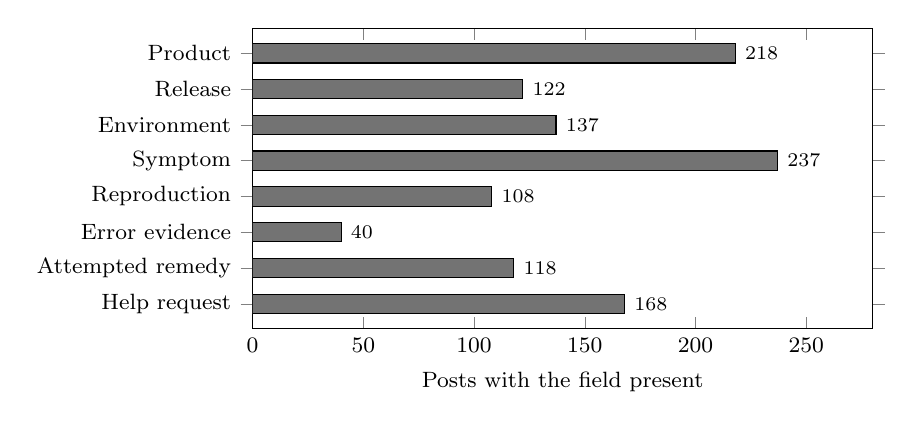
\begin{tikzpicture}
\begin{axis}[
    xbar,
    width=0.78\columnwidth,
    height=5.4cm,
    xmin=0, xmax=280,
    xlabel={Posts with the field present},
    symbolic y coords={Help,Remedy,Error,Repro,Symptom,Environ.,Release,Product},
    ytick=data,
    yticklabels={Help request,Attempted remedy,Error evidence,Reproduction,Symptom,Environment,Release,Product},
    y tick label style={font=\footnotesize},
    x tick label style={font=\footnotesize},
    xlabel style={font=\footnotesize},
    nodes near coords={\pgfmathprintnumber{\pgfplotspointmeta}},
    every node near coord/.append style={font=\scriptsize, /pgf/number format/fixed},
    bar width=7pt,
]
\addplot[fill=black!55] coordinates {(168,Help) (118,Remedy) (40,Error) (108,Repro) (237,Symptom) (137,Environ.) (122,Release) (218,Product)};
\end{axis}
\end{tikzpicture}
\caption{Present counts from Table~\ref{tab:fields}. The symptom count follows reconfirmation. Seven unclear error-evidence decisions are omitted rather than treated as absence.}
\label{fig:fields}
\end{figure}

\subsection{Purpose is not the first action}
The two reviewers chose the same first action in 21 of the 30 cases and different actions in nine. Both chose investigation in ten cases, clarification in six, monitoring in one, and no update-focused action in four. One reader selected investigation 16 times and the other 11 times; the second selected monitoring five times and the first once. In the nine disagreements, the written explanations often cited overlapping facts and differed on whether those facts were sufficient to act, which question should come first, or whether wider impact was established. One post assigned to other update discussion led both readers to investigate. These contrasts show that a purpose label is not an action key. The written explanations add three boundary patterns, stated here without post identifiers. Concrete update-linked failures, together with a comparison or a recovery impact, could support investigation in some of these cases. A concrete symptom did not always settle the next action: in one browser-crash case both reviewers wanted a normal-versus-private-window comparison first, and in one storage case both wanted the space measurement clarified. A reported workaround did not map to one action. Both reviewers opened a lead for one editor case that already had a workaround, whereas in two other cases one reviewer opened a lead and the other preferred monitoring. Some dissatisfaction-labeled posts described concrete changed behavior and still led to different actions.

\section{Discussion}
Three separations follow from the results, and none of them is a pipeline.

\begin{figure}[t]
\centering
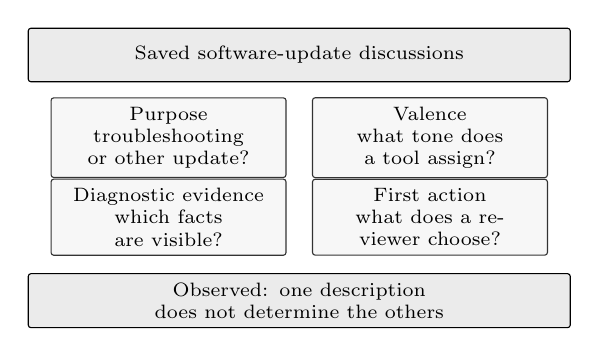
\begin{tikzpicture}[
  font=\scriptsize,
  lens/.style={draw=black!80, fill=black!3, align=center,
    rounded corners=1pt, text width=2.75cm, minimum height=0.73cm},
  finding/.style={draw=black, fill=black!8, align=center,
    rounded corners=1pt, text width=6.65cm, minimum height=0.68cm}
]
\node[finding] (post) at (0,0) {Saved software-update discussions};
\node[lens] (purpose) at (-1.66,-1.05) {Purpose\\troubleshooting or other update?};
\node[lens] (tone) at (1.66,-1.05) {Valence\\what tone does a tool assign?};
\node[lens] (facts) at (-1.66,-2.06) {Diagnostic evidence\\which facts are visible?};
\node[lens] (action) at (1.66,-2.06) {First action\\what does a reviewer choose?};
\node[finding] (lesson) at (0,-3.12) {Observed: one description does not determine the others};
\end{tikzpicture}
\caption{Four complementary readings of software-update discussion. The four boxes represent separate analyses on different subsets, not stages of an implemented or evaluated triage system.}
\label{fig:framework}
\end{figure}

First, the valence gap depends on both the comparison class and the sentiment tool. Under VADER, troubleshooting text is more negative than the broad other-update class on average, but indistinguishable in mean from the 68 posts labeled dissatisfaction. Under SentiStrength-SE, those 68 posts score substantially more negative than troubleshooting. This exploratory tool contrast does not identify which score better captures human sentiment; there is no sentiment gold standard here. It shows why a pooled ``sentiment versus troubleshooting'' graph can conceal both class composition and tool choice. The secondary cohort, whose negative class is assigned dissatisfaction, can still show an author-track difference. That result belongs to its own labels and does not license pooling the 542 with the 2,050.

Second, the purpose classifier and a sentiment score are not substitutes, and the comparison is not only a bake-off among sentiment tools. Title and body text beats majority and fixed-keyword baselines on the fresh test, including a lower other-update F1 of 0.667 that should stay visible next to the headline 0.792. Title alone and body alone are both lower on the development folds, and those grouped intervals exclude zero. VADER, TextBlob, and SentiStrength-SE alone score above majority but far below title and body. The contextual score alone is higher than those three and still below title and body. Adding any of the four scores leaves a grouped interval that includes zero. The frozen MiniLM point estimate is higher, and its interval also includes zero, so this paper does not rank it above the TF--IDF model. Adding sentiment columns to a full thread, on the minority of posts that have comments, lowers macro-F1 in this sample. That lower score is reported because it is what the comparison produced. It is not evidence that sentiment is generally harmful, and it is not evidence that a comment fixed an issue. The practical reading is narrower: for this purpose task, the useful signal in the saved text is not well summarized by a valence score.

The fine-tuned RoBERTa comparator is also slightly higher on development macro-F1, but its paired interval includes zero; it is more expensive to train, truncates some posts, and has not been tested on the protected cohorts. Thus it does not justify replacing the simpler classifier for this paper. The fold-wise terms make that result more interpretable, but also expose a threat: product and platform vocabulary can act as a shortcut when source communities and assigned classes are entangled. A high coefficient for a word is not proof of a generalizable troubleshooting concept. The fresh test and source-aware error analysis therefore matter more than a plausible-looking term list.

Third, detecting troubleshooting does not decide what an engineer should do next. In the 237 confirmed posts, a product name is usually visible and a specific symptom was required by reconfirmation, but error evidence and reproduction context are often not in the snapshot. Twenty confirmed posts have no body at all, and those 20 account for half of the 16 development misses in the exploratory join. In the 30 intact cases, reviewers sometimes chose different first actions from overlapping facts, and one post outside the troubleshooting class still drew investigation from both. Purpose classification can organize a queue. It does not certify that the snapshot is sufficient, and it does not replace the judgment the two reviewers recorded.

\section{Threats}
The collection comes from candidate routes plus assigned labels, not a random sample of Reddit. Thirty records have non-Reddit URL metadata and are excluded from the primary results. The fresh and reserved scores belong to separate fits of the same specification and were not recomputed for the new development arms. The RoBERTa comparison is development-only; 442 inputs are truncated at 256 tokens, and its fold-specific thresholds vary from 0.35 to 0.80. Comment missingness differs by class, and both-role coverage is below the predeclared bar. VADER returns zero for an empty document. The contextual checkpoint is a social-media model, and 188 development texts were truncated at 512 tokens. SentiStrength-SE was developed for software-engineering interactions, not specifically for Reddit update reports. Its signed strengths were reduced to one scalar; a different representation could behave differently. Its 68-post dissatisfaction contrast was examined after the main tool comparison and is exploratory. Senti4SD could not be scored because its required pretrained files were unavailable. There is no independent sentiment gold label. The technical-word lists were fixed before counting and exclude the words ``update'' and ``upgrade'' because the collection is update-scoped; they are not a masking experiment. Diagnostic coding has one joint review record. The 30 cases were purposefully varied. The four paraphrased errors are illustrations, not a coded error taxonomy. No causal effect of sentiment, fields, or the classifier on engineering work is identified.

\section{Future Work}
The next study should test whether the four descriptions help engineers perform a real first-pass triage task, with outcomes such as time to a justified decision and the usefulness of requested clarifications. That requires more independent reviewers and prospective evaluation; the 30 cases here cannot establish those outcomes. GitHub issues, Jira tickets, and Stack Overflow questions would test whether the distinctions survive different authors, fields, and moderation practices. A deployed monitor would also need to measure collection delay, comment availability, and shifts across releases before any claim about real-time issue discovery. Language-model assistance could suggest a missing diagnostic question, but its suggestions would need human verification against the source text and should be evaluated for unsupported details. These are proposed tests, not results of this study.

\section{Conclusion}
An informal update post can express a negative reaction, describe a fault, supply diagnostic facts, and suggest an engineering response, but those are different claims about the post. Title-and-body text identifies troubleshooting on a fresh Reddit-URL test at macro-F1 0.792. In the grouped development comparison, adding any of four tested valence scores, including SentiStrength-SE, gives no reliable improvement over that text. The apparent tone gap depends on both the comparison class and the scoring tool. Among confirmed troubleshooting posts, diagnostic facts such as reproduction context and error evidence are often not visible; two readers of the same 30 intact posts disagreed on nine first actions. The scientific contribution is this measured boundary between recognizing a report and knowing what to do with it. A useful future triage aid should preserve that boundary, surface the evidence behind each suggestion, and let an engineer decide what information is still needed.

\section*{Acknowledgment}
OpenAI Codex assisted with research planning, source audits, literature checks, and manuscript review. Cursor assisted with drafting, LaTeX, tables, and figures from saved results. The authors verified the claims, citations, and final wording. Neither tool created human labels, diagnostic codes, or reviewer decisions. We disclose this assistance under IEEE's author guidelines \cite{IEEE2024AIText}.

\bibliographystyle{IEEEtran}
\bibliography{references}
\end{document}
